\documentclass[varwidth=true]{standalone}
\usepackage{graphicx}
\usepackage{tikz}
% Tikz libraries
\usetikzlibrary{%
    patterns, plotmarks, backgrounds, shapes, arrows, calc, trees, positioning,
    chains, shapes.geometric, decorations.pathreplacing,
    decorations.pathmorphing, shapes.arrows, decorations.markings, quotes, 
    shapes.geometric, arrows.meta, spy, fit, matrix, math, bending, graphs,
    graphs.standard, through
}

% Captions and subcaptions
\usepackage{xcolor}
\usepackage{subcaption}
\captionsetup{justification=raggedright,singlelinecheck=false,labelsep=space}
\usepackage[labelformat=simple]{subcaption}
\renewcommand\thesubfigure{(\alph{subfigure})}
\usepackage{amsmath}
\renewcommand{\familydefault}{\sfdefault}

\begin{document}

\begin{figure}
     \begin{subfigure}[t]{1.0\textwidth}
        \caption{Phenylalanine transaminase}
        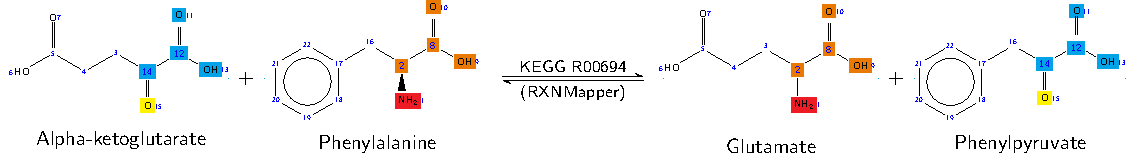
\includegraphics[width=1.0\textwidth]{phenylalanine-transaminase-incorrect.pdf}
        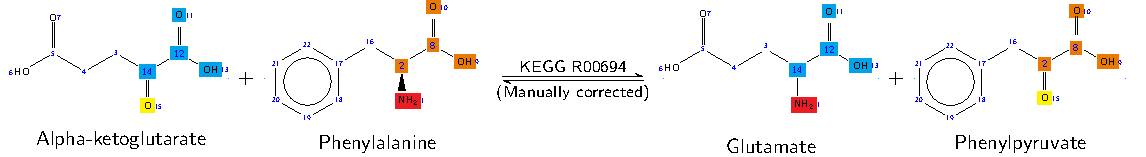
\includegraphics[width=1.0\textwidth]{phenylalanine-transaminase-correct.pdf}
        \caption{Isoleucine transaminase}
        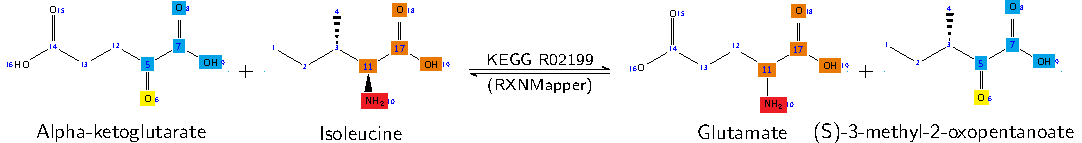
\includegraphics[width=1.0\textwidth]{isoleucine-transaminase-incorrect.pdf}
        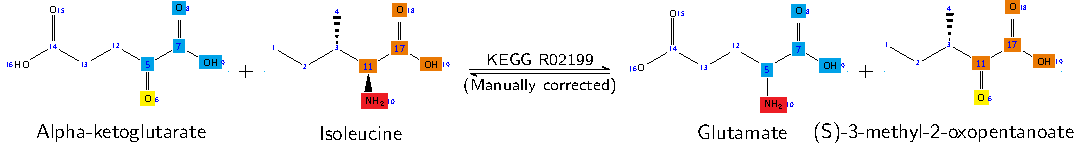
\includegraphics[width=1.0\textwidth]{isoleucine-transaminase-correct.pdf}
        \caption{Leucine transaminase}
        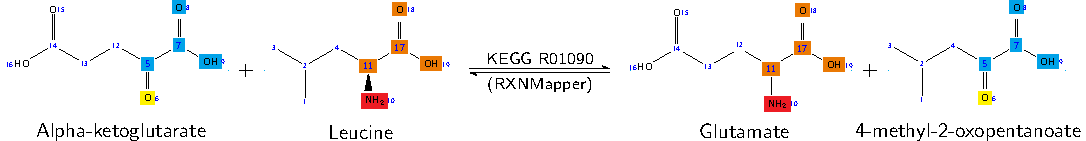
\includegraphics[width=1.0\textwidth]{leucine-transaminase-incorrect.pdf}
        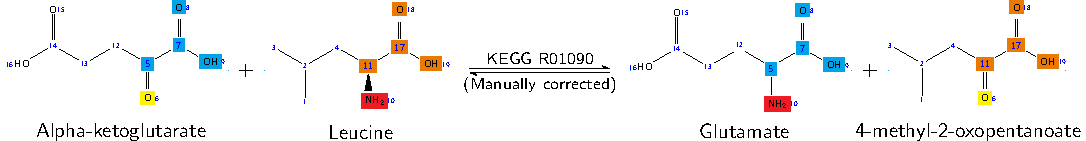
\includegraphics[width=1.0\textwidth]{leucine-transaminase-correct.pdf}
        \caption{Tyrosine transaminase}
        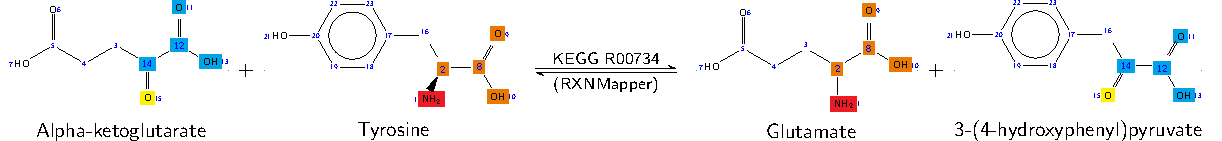
\includegraphics[width=1.0\textwidth]{tyrosine-transaminase-incorrect.pdf}
        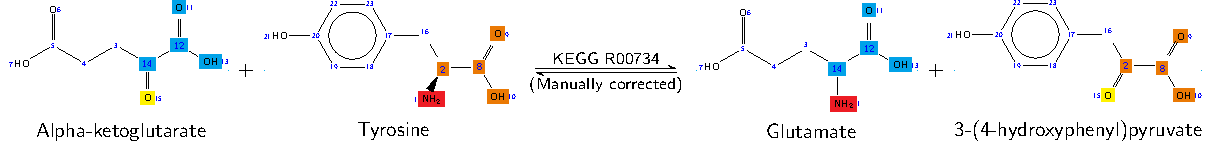
\includegraphics[width=1.0\textwidth]{tyrosine-transaminase-correct.pdf}
        \caption{Phosphoserine transaminase (redo)}
        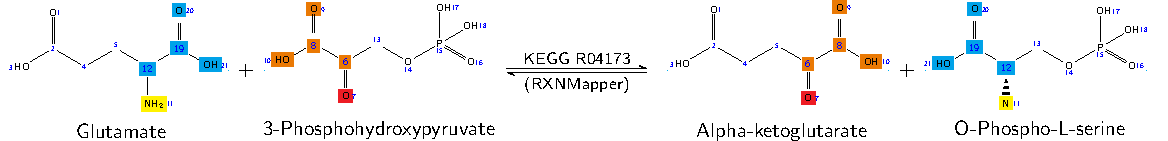
\includegraphics[width=1.0\textwidth]{phosphoserine-transaminase-incorrect.pdf}
        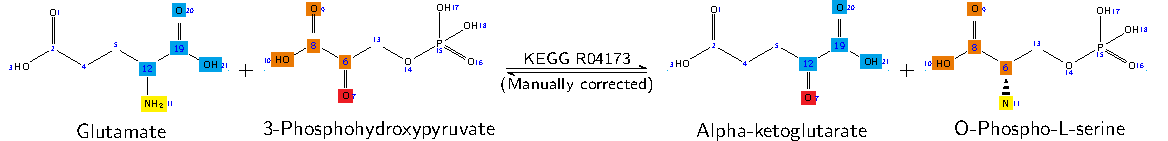
\includegraphics[width=1.0\textwidth]{phosphoserine-transaminase-correct.pdf}
        \caption{Valine transaminase}
        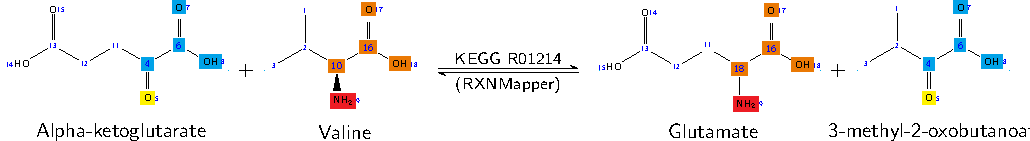
\includegraphics[width=1.0\textwidth]{valine-transaminase-incorrect.pdf}
        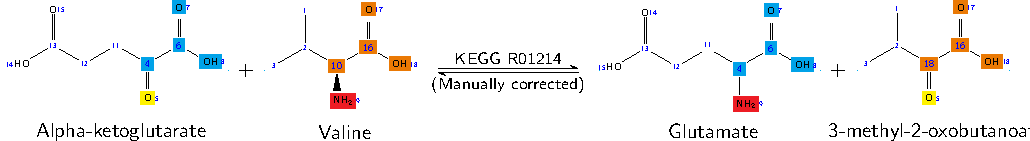
\includegraphics[width=1.0\textwidth]{valine-transaminase-correct.pdf}
        \caption{Aspartate transaminase}
        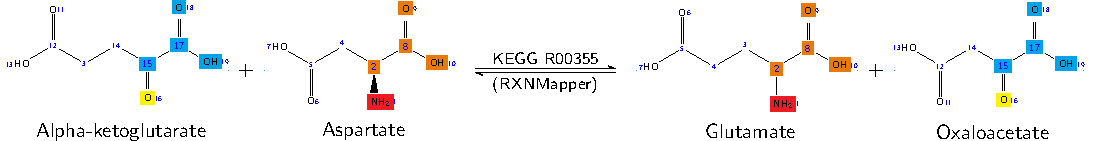
\includegraphics[width=1.0\textwidth]{aspartate-transaminase-incorrect.pdf}
        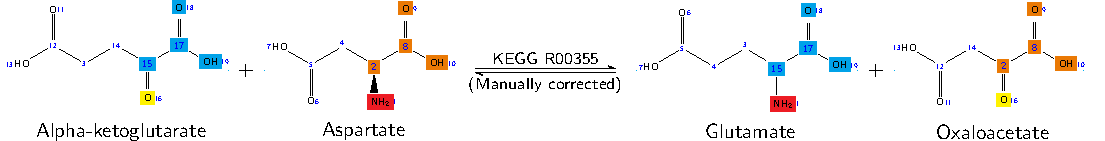
\includegraphics[width=1.0\textwidth]{aspartate-transaminase-correct.pdf}
    \end{subfigure}
\end{figure}

\end{document}

